\chapter{Our solution} \label{our:solution}


% uvod, co je v kapitole, nejdriv...
% obecne algorithmus bez rozzepsaneho gpcka

% Prvni cats - GPcko (zakodovani, init, operat., fitness jak se pocita (ale vic dole),...
% Druha - Sklearn strana, eval, samples,...

% Posledni- implementace, deap,...

% experimenty 4

In our solution we design an AutoML system for workflow optimization based on
developmental genetic programming. Compared to existing systems it supports 
arbitrary-sized pipelines as well as complex ensemble structures. We first
present in what way we use the genetic programming, then we describe the
pipeline evaluation process.

\section{Evolutionary optimization of pipelines}
The algorithm corresponds to the schema of a general genetic algorithm
\ref{alg:EA}. In this section we describe the necessary components of the
algorithm.

\subsection{Individual encoding}
The individual encoding is one of the most important parts of this system. With
ensembles and complex feature preprocessing methods like stacking or feature
union, most of the pipelines become in fact directed acyclic graphs (figure 
\ref{pic02:pipeline}). Therefore, we cannot directly use the simple tree-based
encoding. Instead we use the developmental GP with cellular encoding described
in section \ref{devGP}.
\begin{figure}[ht]\centering
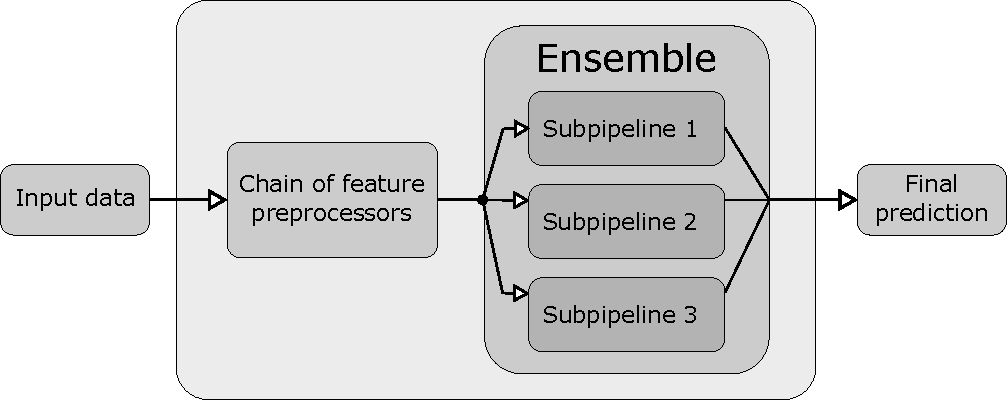
\includegraphics[width=0.7\textwidth]{../img/pipeline-pdfa.pdf}
\caption{Schema of an example pipeline}
\label{pic02:pipeline}
\end{figure}

In our case, the embryo is an empty pipeline. To create a complex pipeline, we
modify it by inserting steps into it.

\begin{figure}[ht]\centering
    \subfloat[Tree encoding]{{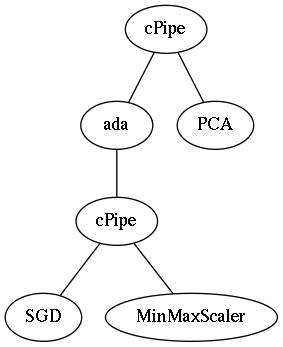
\includegraphics[width=0.25\textwidth]{../img/ada.png} }}%
    \qquad
    \subfloat[Encoded pipeline]{{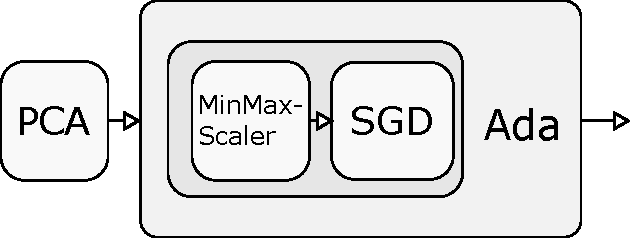
\includegraphics[width=0.5\textwidth]{../img/ada-pdfa.pdf} }}%
    \caption{An example pipeline encoded to a tree individual}%
    \label{pic:pipeencoding}%
\end{figure}

The process can be demonstrated on figure
\ref{pic:pipeencoding}. The root of the tree represents the embryo which will
be modified by subsequent operations. In this case, the left subtree modifies
the ensemble structure whereas the right subtree modifies the feature
preprocessor chain. The pipeline contains only one preprocessor, hence the
right subtree is terminated by the corresponding node. The left son can be
either an ensemble or a simple method. Here it is the AdaBoost ensemble which
has one base classifier. The subestimator is again a pipeline, which is composed
of a MinMaxScaler and Stochastic gradient descent classifier. The specific
hyperparameter of every pipeline step are stored aside the nodes and are not
depicted in the figures.

Table \ref{tab03:nodes} lists the nodes used in the current implementation of
our system. Input type is defined as a cartesian product of types, output type
is a single type; terminals have only the output type defined. Output types of
child nodes must match the input type of parent node. The list is extensible,
it is possible to add a definion of similar nodes, e.g. a different ensemble
flavour like stacking. The nodes that are specific for a given estimator
correspond to the list of methods in section \ref{tab03:methods}.

% TODO should I describe node types?
\begin{table}[b!]

\centering
\begin{tabular}{l c c p{0.38\textwidth}}
\toprule
\mc{\textbf{Node}\textsuperscript{1}} & \mc{\textbf{In type}\textsuperscript{2}} &
\mc{\textbf{Out type}\textsuperscript{3}} & \mc{\textbf{Operation}} \\
\midrule
cPipe       & $ens \times data$      & $out$  & Create pipeline with a preprocessor chain and a predictor \\
cPred       & $ens$                  & $out$  & Create pipeline only with a predictor \\
cData       & $featsel \times scale$ & $data$ & Create preprocessor chain with feature selector and scaler \\
cFeatSelect & $featsel$              & $data$ & Create preprocessor chain only with a feature selector \\
cScale      & $scale$                & $data$ & Create preprocessor chain only with a scaler \\
dUnion      & $data^n$               & $data$ & Create feature union in the preprocessor chain \\
\textit{ensemble} & $out^n$ & $ens$ & Insert ensemble \\
\textit{classifier} & $\emptyset$ & $out$ & Insert classifier \\
\textit{selector} & $\emptyset$ & $featsel$ & Insert feature selector \\
\textit{scaler} & $\emptyset$ & $scale$ & Insert scaler \\
\bottomrule

\multicolumn{4}{l}{\footnotesize
\textsuperscript{1}\textit{There is one specific node per ensemble, classifier
and preprocessor present}} \\

\multicolumn{4}{l}{\footnotesize
\textsuperscript{2}\textit{Variable arity is allowed (i.e. $n \in <1, max\_n>)$}} \\

\multicolumn{4}{l}{\footnotesize
\textsuperscript{3}\textit{In the last level classifier and preprocessing
can have output type $ens$ and $data$ resp.}} 

\end{tabular}
\caption{Nodes representing modifying operations}\label{tab03:nodes}

\end{table}

\subsection{Initialization}
As the initial population we grow $n$ trees where every tree has a random
height between 1 and overall maximum height. The tree is grown from root, which
is either a 'cPipe` or 'cPred` node (table \ref{tab03:nodes}). Then, nodes are
inserted into the tree according to the input type of the parent. Before the
height limit is reached (during the \emph{growing phase}), both functions and
terminals are inserted into the tree. Then, only terminals are inserted to
keep the limit.

As terminals are inserted in the growing phase as well, the tree may become
smaller than the height limit. However, if the tree were built using the full
method, it would introduce a lot of feature preprocessing methods for taller
trees. Therefore, all node types listed in table \ref{tab03:nodes} may be used
during the growing phase. Moreover, we define special terminal nodes which are
used only in the last level (\hyperref[tab03:nodes]{footnote 2}). It is
necessary to include them, as otherwise it would be impossible to finish the
tree in one level, but they would force the trees to be very short if used
during the growing phase.

\paragraph{Weighted selection}
During the node selection, we use weights to manage the probability of a node
to be chosen. The motivation is that some nodes represent lightweight methods
which have a short execution time, whereas some nodes slow down the evaluation
process, especially when present multiple times in the tree.

The process is as follows: every node is assigned to a group and each group has
a well defined weight. When selecting a node $n$ with output type $out$, we 
first determine all groups $G$ which correspond to any node with output type
$out$. Then we select a group $g$ from $G$ by a weighted random choice.
Finally, $n$ is selected by a simple random choice from $g$.

\paragraph{Variable arity}
Some nodes, e.g. ensemble nodes, may have a \emph{variable arity}. This means
that the actual arity is determined just when the node is about to be inserted
to the tree. The arity is determined by an interval which may or may not have
an upper bound. If the upper bound is not provided, it is usually limited by
a global arity limit to avoid bloat of the trees.

\paragraph{Method hyperparameters}
Every node has a list of possible values per hyperparameter associated with
it. During selection, the actual values are randomly selected from every list.
The validity is not verified in this phase, instead it is handled in the
evaluation phase \ref{sec:eval}.

\subsection{Genetic operators}
In our system we use one type of crossover and three different types of
mutation. The crossover is the standard strongly typed subtree-swap operation.
The mutation operators will be described in more detail.

\paragraph{Subtree mutation}
As defined in section \ref{treeops}, in subtree mutation a chosen subtree is
replaced with a randomly generated tree. In our implementation we moreover
limit the height of the generated tree. For height $h$ of the subtree, the
height of the newly generated tree must be between $<1, h + \epsilon>$ for a
small value of $\epsilon$. This way we ensure that for small subtrees the new
subtree may be slightly higher and for big subtrees the overall height should
not increase too much.

\paragraph{Node swap mutation}
In this type of mutation, a randomly chosen node is replaced with a new node.
Both output and input types must match; if the new node supports variable
arity, all input types of the old node must satisfy the bounds. For this type
of mutation, any lower bound must be greater than zero.

\paragraph{Node argument mutation}
Mutates a hyperparameter of a random node --- chooses a new value from the list
of possible values. Has many possible extensions which are more described in
section \ref{future} (future work).

\subsection{Fitness and selection}

The fitness has two objectives --- evaluation score and evaluation time. The
enviromental selection is done via NSGA-II and the parental selection is a
tournament selection based on individual dominance and crowding distance.
Details about method implementations are provided in section \ref{sec:eval}.

\section{Evaluation and performance estimation} \label{sec:eval}
In this section we elaborate the evaluation process. First we present the
pipelines and used methods in more detail. Then we present a performance
estimation method which was used to decrease the running time.

\subsection{Used machine learning methods}

\subsection{Scoring and sampling}
Fitness evaluation is the major performance\ldots
% zabira nejvic casu, je hlavni polozkou, nevim jak to napsat
The long running time is one of the drawbacks of evolution-based systems. On
large datasets, the evolution time may be too long even for a small number of
populations of small size. As such, it is necessary to decrease the evaluation
time of a single individual. We use one of the performance estimation methods
mentioned in section \ref{sec:modelarch} --- evaluation on smaller subsets of
data.

\section{Implementation}